\subsection{GPQA: A Graduate-Level Google-Proof Question and Answer Benchmark}
{{\footnotesize
\noindent Contains 448 challenging questions written by domain experts, with expert accuracy at 65\% (74\% discounting clear errors) and non-experts reaching just 34\%. GPT-4 baseline scores \textasciitilde{}39\%-designed for scalable oversight evaluation. 


\begin{description}[labelwidth=4cm, labelsep=1em, leftmargin=4cm, itemsep=0.1em, parsep=0em]
  \item[date:] 2023-11-20
  \item[version:] v1.0
  \item[last\_updated:] 2023-11
  \item[expired:] unknown
  \item[valid:] yes
  \item[valid\_date:] 2023-11-20
  \item[url:] \href{https://arxiv.org/abs/2311.12022}{https://arxiv.org/abs/2311.12022}
  \item[doi:] 10.48550/arXiv.2311.12022
  \item[domain:]
    - Biology \& Medicine
    - High Energy Physics
    - Chemistry
  \item[focus:] Graduate-level, expert-validated multiple-choice questions hard even with web access
  \item[keywords:]
    - Google-proof
    - multiple-choice
    - expert reasoning
    - science QA
  \item[licensing:] NA
  \item[task\_types:]
    - Multiple choice
  \item[ai\_capability\_measured:]
    - Scientific reasoning
    - knowledge probing
  \item[metrics:]
    - Accuracy
  \item[models:]
    - GPT-4 baseline
  \item[ml\_motif:]
    - Reasoning \& Generalization
  \item[type:] Benchmark
  \item[ml\_task:]
    - Multiple choice
  \item[solutions:] Solution details are described in the referenced paper or repository.
  \item[notes:] Google-proof, supports oversight research.

  \item[contact.name:] David Rein (NYU)
  \item[contact.email:] unknown
  \item[datasets.links.name:] GPQA dataset
  \item[datasets.links.url:] \href{zip/HuggingFace}{zip/HuggingFace}
  \item[results.links.name:] ChatGPT LLM
  \item[fair.reproducible:] Yes
  \item[fair.benchmark\_ready:] Yes
  \item[id:] gpqa\_a\_graduate-level\_google-proof\_question\_and\_answer\_benchmark
  \item[Citations:] \cite{rein2023gpqagraduatelevelgoogleproofqa2}
\end{description}

{\bf Ratings:} ~ \\

\begin{tabular}{p{0.15\textwidth} p{0.07\textwidth} p{0.7\textwidth}}
\hline
Rating & Value & Reason \\
\hline
dataset & 5 & The GPQA dataset is publicly released, well curated, with metadata and clearly documented splits.
 \\
documentation & 3 & Documentation includes dataset description and benchmark instructions, but lacks detailed usage tutorials or pipelines.
 \\
metrics & 5 & Accuracy is the primary metric and is clearly defined and appropriate for multiple-choice QA.
 \\
reference\_solution & 1 & No baseline implementations or starter code are linked or provided for reproduction.
 \\
software & 3 & Dataset and benchmark materials are publicly available via HuggingFace and GitHub,
but no integrated runnable code or software framework is provided.
 \\
specification & 5 & Task is clearly defined as a multiple-choice benchmark requiring expert-level scientific reasoning.
Input/output formats and evaluation criteria are well described.
 \\
\hline
\end{tabular}

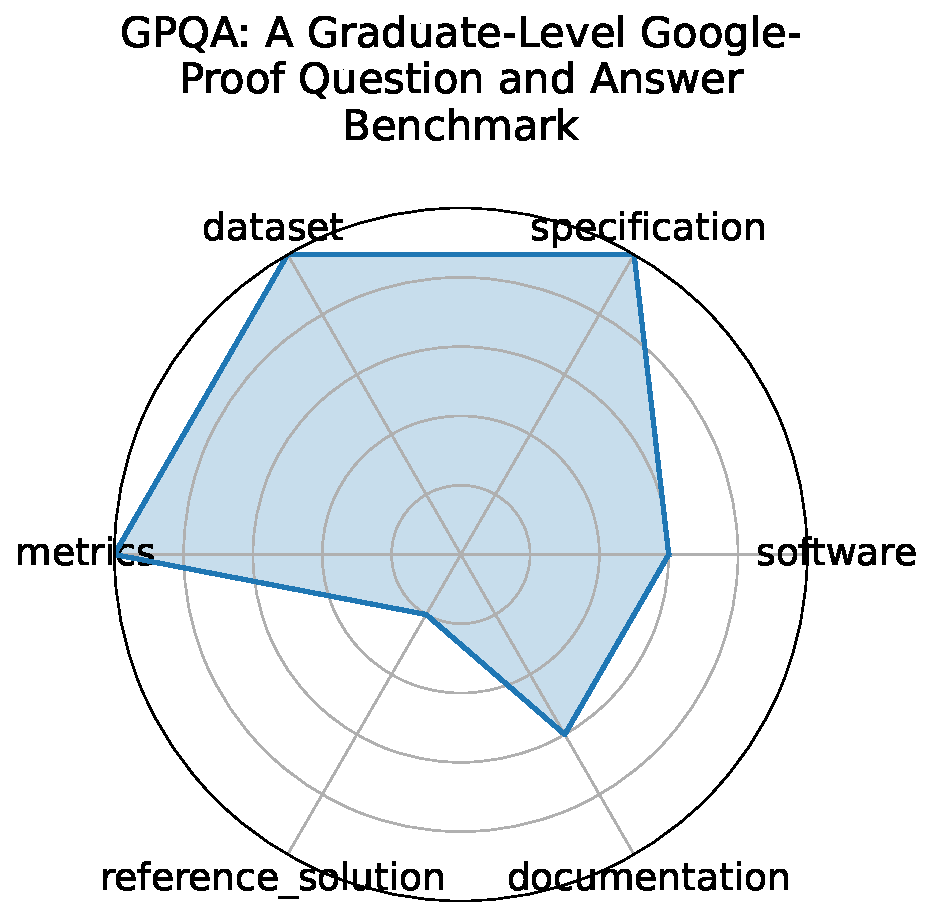
\includegraphics[width=0.2\textwidth]{gpqa_a_graduate-level_google-proof_question_and_answer_benchmark_radar.pdf}
}}
\clearpage